\documentclass{article}
\usepackage[utf8]{inputenc}

\usepackage{geometry}
\geometry{
  paper=a4paper,
  margin=1in,
}

\usepackage{amsmath,amsthm,amsfonts}
\usepackage{url}
\usepackage{hyperref}

\usepackage{graphicx}

\usepackage{mathtools}
\usepackage{centernot}

\usepackage[shortlabels]{enumitem}


\theoremstyle{plain}
\newtheorem{thm}{Theorem}[section]
\newtheorem{lem}[thm]{Lemma}
\newtheorem{prop}[thm]{Proposition}
\newtheorem{cor}[thm]{Corollary}
\newtheorem{conj}[thm]{Conjecture}

\theoremstyle{definition}
\newtheorem{definition}[thm]{Definition}


\usepackage{tcolorbox}

\newtheorem{exmp}{Example}[section]
\newtheorem*{sol}{Solution}

\numberwithin{equation}{section}

\newcommand*{\colorboxed}{}
\def\colorboxed#1#{%
  \colorboxedAux{#1}%
}
\newcommand*{\colorboxedAux}[3]{%
  % #1: optional argument for color model
  % #2: color specification
  % #3: formula
  \begingroup
    \colorlet{cb@saved}{.}%
    \color#1{#2}%
    \boxed{%
      \color{cb@saved}%
      #3%
    }%
  \endgroup
}


% \setcounter{section}{-1}

\title{Mathematical Methods}
\author{Iain McWhinnie}
\date{December 2022}

\begin{document}

\maketitle

\tableofcontents

\section{Second Order Linear Differential Equations}

\subsection{Introduction}

In this chapter we aim to find solutions to 2nd order linear differential equations.

\begin{definition}
A general \textbf{second order ODE} has the form
\[
y'' = f(t,y,y')
\]
where $y$ is the unknown function and $f: \mathbb{R}^3 \mapsto \mathbb{R}$ is given.


The \textbf{order} of the differential equation  is the highest derivative appearing in the ODE. The equation is \textbf{linear} if the function $f$ is linear in both arguments $y$ and $y'$ i.e.,
\[
f(t,y,y') = a(t)y + b(t)y' + c(t).
\]

\end{definition}

\begin{definition}
    A second order \textbf{linear} differential equation in the unknown $y$ is
    \begin{equation}
        a(t)y'' + b(t)y' + c(t) = h(t)
    \end{equation}
    where $a,b,c,h: I \mapsto \mathbb{R}$ are given functions on the interval $I \subseteq \mathbb{R}$. 
    
    The equation is called \textbf{homogeneous} if the source term $h(t)=0$ for all $t\in I$. The equation is called \textbf{constant coefficient} if $a(t), b(t)$ and $c(t)$ are constants otherwise the equation is called \textbf{variable coefficient}.

\end{definition}

\begin{tcolorbox}
\begin{exmp}\hfill
\begin{enumerate}[(a)]
    \item A second order linear homogeneous constant coefficient equation is
    $$ y'' + 5y' + 6y = 0.$$
    \item A second order linear inhomogeneous constant coefficient equation is
    $$ y'' - 3y' + y = \cos(3t).$$
    \item A second order linear inhomogenouse variable coefficient equation is
    $$ y'' - 2ty' - \ln(t)y = e^{3t}.$$
    \item Newton's second law of motion for a point particle of mass $m$, moving in one space dimensions under a force $f$ is given by
    $$ my'' = f(t)$$
    ($\text{force} = \text{mass} \times \text{acceleration}$).
\end{enumerate}
\end{exmp}
\end{tcolorbox}

\subsection{Initial Value Problems}

\begin{thm}[Existence and Uniqueness]\label{thm:Existenceanduniqueness}
If the functions $p(t),q(t),f(t):I \mapsto \mathbb{R}$ are continuous on a closed interval $I \subseteq \mathbb{R}$ and $t_0 \in I$ and $b_0,b_1 \in \mathbb{R}$ are constants, then there \textbf{exists} a \textbf{unique} solution $y: I \mapsto \mathbb{R}$ to the \textbf{initial value problem} (IVP)
\begin{equation}\label{eq:linearIVP}
\left.
\begin{aligned}
    y'' + p(t)y' + q(t)y = f(t) \\
    y(t_0) = b_0, \quad y'(t_0) = b_1 \\
\end{aligned}\quad\right\rbrace
\end{equation}
\end{thm}

\begin{proof}
    Omitted. It is actually an application of the contraction mapping theorem from metric spaces.
\end{proof}

\begin{figure}[h]
    \centering
    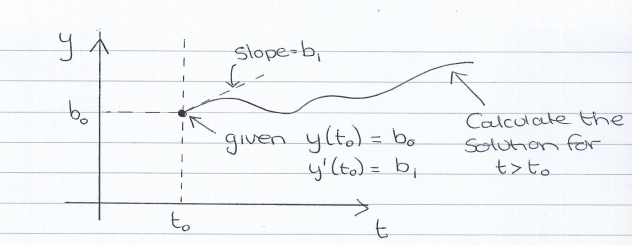
\includegraphics{images/Ivpgraph.png}
    \caption{An initial value problem.}
    \label{fig:ivpgraph}
\end{figure}

\begin{tcolorbox}
\begin{exmp}
Find the largest interval $I \in \mathbb{R}$ such that there exists a unique solution to the IVP:
\[
\begin{aligned}
    (t-1)y'' - 3ty' + 4y = t(t-1) \\
    y(-2) = 2, \quad y'(-2) = 1 \\
\end{aligned}
\]
\end{exmp}
\begin{sol}
    Rewriting the ODE in the form of Theorem \ref{thm:Existenceanduniqueness} we have
    \[
    y'' - \frac{3t}{t-1}y' + \frac{4}{t-1}y = t.
    \]
    The intervals where $\frac{3t}{t-1}, \frac{4}{t-1}$ and $t$ are all continuous are
    \[
        I_1 = (-\infty, 1) \quad \text{and} \quad I_2 = (1, \infty).
    \]
    Since the initial condition lies in the interval $I_1$ the solution domain is
    \[
        I_1 = (-\infty, 1).
    \]
\end{sol}
\end{tcolorbox}

We will look at an example of a homogeneous equation with constant coefficients

\begin{tcolorbox}
\begin{exmp}
    Solve $y''+5y' + 6y = 0$ with $y(0)=2$ and $y'(0)=3$.
\end{exmp}
\begin{sol}
    We try a solution of the form $y(t)=\exp(\lambda t)$ to derive the auxiliary equation
    \[
    \lambda^2 + 5\lambda + 6 =9
    \]
    which factors to give $(\lambda + 2)(\lambda + 3) = 0$. Hence $\lambda = -2$ or $\lambda = -3$.

    The general solution is then
    \[
        y(t) = c_1 e^{-2t} + c_2 e^{-3t},  
    \qquad c_1,c_2 \in \mathbb{R}.
    \]
    Applying the initial conditions we find that
    \[
    \left.
    \begin{aligned}
        y(0) = 2 = c_1 + c_2 \\
        y'(0) = 3 = 2c_1 - 3c_2 \\
    \end{aligned}
    \quad\right\rbrace
    \]
    Hence $c_1 = 9$ and $c_2 = -7$ so the unique solution to the IVP is
    \[
        y(t) = 9e^{-2t} - 7e^{-3t}.
    \]
\end{sol}
\end{tcolorbox}

This leaves us with a few questions
\begin{enumerate}[(i)]
    \item Why did we add the two solutions together to get the general one?
    \item Why is this the general solution?
    \item What would the solution to the more general ODE \eqref{eq:linearIVP} look like?
\end{enumerate}

To answer these questions it is useful to introduce the definition of an operator, we will do this in the next section.

\subsection{Linear Operators}

A function $f: \mathbb{R} \mapsto \mathbb{R}$ takes a number as an input and produces another number as an output
\[
    x \ \xlongrightarrow{\quad\textit{f}\quad} \ f(x)
\]
i.e.,
\[
    \text{number}\ \xlongrightarrow{\quad\textit{f}\quad} \ \text{another number}.
\]
A simple example is $f(x) = x^2$ which maps
\[
    x \ \xlongrightarrow{\quad\textit{f}\quad}  \ x^2.
\]
One can thing of differentiating in a similar way but with the inputs and outputs as functions rather than numbers, i.e.,
\[
    \text{function}\ \xlongrightarrow{\text{operator}}\ \text{another function}.
\]
For example,
\[
    y(t)\ \xlongrightarrow{\quad\textit{L}\quad} \ y'' + y
\]
here $L = \frac{d^2}{dt^2} + 1$. $L$ is called an \textbf{operator} or \textbf{functional}.

\begin{tcolorbox}
\begin{exmp}
    Let $L = \frac{d}{dx} + x^2$, then $L$ sends the function $y(x)$ to the function $\frac{dy}{dx} + x^2y$.

    We use square brackets $L[y]$ to denote the output of the operator so
    \[
        L[y] = \frac{dy}{dx} + x^2y.
    \]
    The new function $L[y]$ can be evaluated at a number $x$, this is denoted by
    $$ L[y(x)] \quad \text{or} \quad L[y](x).$$
    So for example
    \begin{align*}
        L\left[\sin(x)\right] &= \frac{d}{dx}\left( \sin x \right) + x^2 \sin x \\
        &= \cos x + x^2 \sin x. \\
    \end{align*}
\end{exmp}
\end{tcolorbox}

Let us consider the operator
\begin{equation*}
    L[y] = y'' + p(t)y' + q(t)y
\end{equation*}
then equation \eqref{eq:linearIVP} can be written as $L[y] = f$.

\bigskip
A particularly important type of operators are linear operators.

\begin{definition}
    An operator $L$ is called a \textbf{linear operator} if for every pair of function $y_1$ and $y_2$ and constants $c_1,c_2$ we have that
    \[
        L\left[ c_1y_1 + c_2y_2 \right] = c_1 L[y_1] + c_2 L[y_2].
    \]
\end{definition}

\begin{tcolorbox}
\begin{exmp}
    Show that the operator $L = \frac{d^2}{dx^2} + p(t)\frac{d}{dt} + q(t)$ is linear.
\end{exmp}
\begin{sol}
    \begin{align*}
        L[c_1y_1 + c_2y_2] &= \big(c_1y_1 + c_2y_2\big)'' + p(t)\big(c_1y_1 + c_2y_2\big)' + q(t)\big(c_1y_1 + c_2y_2\big) \\
        &= \big(c_1y_1''+p(t)c_1y_1' + q(t)c_1y_1\big) + \big(c_2y_2'' + p(t)c_2y_2' + q(t)c_2y_2\big)\\
        &= c_1 \big( y_1'' + p(t)y_1' + q(t)y_1 \big) + c_2 \big( y_2'' + p(t)y_2' + q(t)y_2 \big) \\
        &= c_1 L[y_1] + c_2 L[y_2] \\
    \end{align*}
    hence $L$ is a linear operator.
\end{sol}

\end{tcolorbox}
\begin{tcolorbox}

\begin{exmp}
    Show that the operator $L[y] = \left(\frac{dy}{dx}\right)^2$ is \textbf{not} linear.
\end{exmp}
\begin{sol}
    \begin{align*}
        L[y_1 + y_2] &= \left(\frac{d(y_1 + y_2)}{dx}\right)^2 = \left( \frac{dy_1}{dx} + \frac{dy_2}{dx} \right)^2 \\
        &= \left(\frac{dy_1}{dx}\right)^2 + 2\frac{dy_1}{dx}\frac{dy_2}{dx} + \left( \frac{dy_2}{dx} \right)^2 \\
        &= L[y_1] + L[y_2] + 2\sqrt{L[y_1]L[y_2]} \\
        & \neq L[y_1] + L[y_2] \\
    \end{align*}
    so $L$ is not a linear operator.
\end{sol}
\end{tcolorbox}
\bigskip
The linearity of an operator $L$ translates to into the superposition property (adding solutions) of the solutions to the homogeneous equation $L[y] = 0$.

\begin{thm}[The Principle of Superposition]
    If $L$ is a linear operator and $y_1,y_2$ are solutions of the homogenenous equations
    \[
        L[y_1] = 0, \quad L[y_2] = 0,
    \]
    then for every constant $c_1,c_2$ we have
    \[
        L[c_1y_1 + c_2y_2] = 0.
    \]
\end{thm}
\begin{proof}
    We verify that $y=c_1y_1 + c_2y_2$ satisfies $L[y] = 0$ for every constant $c_1,c_2.$ We have that
    \begin{align*}
        L[y] &= L[c_1y_1 + c_2y_2] \\
        &= c_1L[y_1] + c_2L[y_2] \\
        &= c_1 \cdot 0 + c_2 \cdot 0 \\
        &= 0
    \end{align*}
    since $L$ is a linear operator.
\end{proof}

\subsection{Linear Dependence of Functions and Wronskians}\label{section:LinearDependence&Wronskians}

We are going to digress away from solutions to ODEs in this section and think about linear dependance of functions.

\begin{definition}
    Two continuous functions $y_1, y_2: I \mapsto \mathbb{R}$ are called \textbf{linearly dependent} on the interval $I \subseteq \mathbb{R}$, if there exists constants $c_1, c_2 \in \mathbb{R}$ not both zero such that for all $t\in I$ we have
    \[
        c_1y_1(t) + c_2y_2(t) = 0.
    \]
    On the contrary, $y_1,y_2$ are \textbf{linearly independent} on the interval $I$ if they are \textbf{not} linearly dependent, that is, the only constants $c_1,c_2$ that for all $t\in I$ satisfy $c_1y_1(t) + c_2y_2(t) = 0$ are the constants $c_1=c_2=0.$
\end{definition}

\begin{tcolorbox}
    \begin{exmp}
        Which of the following pairs of functions are linearly independent?
        \begin{enumerate}[(a)]
            \item $\sin t$ and $\cos(t-\pi/2)$,
            \item $e^t$ and $e^{2t}$.
        \end{enumerate}
    \end{exmp}
    \begin{sol}
        \begin{enumerate}[(a)]
            \item Consider $c_1\sin(t) + c_2 \cos(t-\pi/2) = 0, \quad c_1,c_2 \in \mathbb{R}$. Now by looking at the triangle in Figure \ref{fig:triangle} we can see that $\sin(t) = \cos(t-\pi/2).$

            Therefore by choosing $c_1=-c_2$ we have
            \[
                c_1\sin(t) + c_2 \cos(t-\pi/2) = 0.
            \]
            Thus $c_1,c_2 \neq 0$ and the two function are linearly dependent.
            \item Consider $c_1e^t + c_2e^{2t} = 0, \quad c_1,c_2 \in \mathbb{R}$. Differentiating gives $c_1e^t + 2c_2e^{2t} = 0$. Subtracting one equation from the other gives $c_2e^{2t} = 0$ so $c_2 = 0$. Thus $c_1 = 0$ and therefore the functions are linearly independent.
        \end{enumerate}
    \end{sol}
\end{tcolorbox}

\begin{figure}[htb]
    \centering
    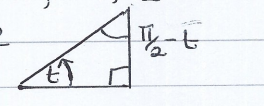
\includegraphics{images/traingle.png}
    \caption{Angles in a right angled triangle}
    \label{fig:triangle}
\end{figure}

\begin{tcolorbox}
\begin{exmp}
    If either function $y_1$ or $y_2$ is the zero function then $y_1,y_2$ are linearly independent. We can show this as follows, let $y_1(t) = 0$ for instance then
    \[
        c_1y_1(t) + 0 \cdot y_2(t) = c_1 \cdot 0 = 0.
    \]
    This is true for any value of $c_2$ therefore there exists $c_1,c_2$ not both zero such that $c_1y_1 + c_2y_2 = 0$.
\end{exmp}
\end{tcolorbox}

\bigskip
\begin{definition}[The Wronskian function]
    The \textbf{Wronskian} of the differentiable functions $y_1,y_2$ is the function
    \[
        W(y_1,y_2) = \left\vert\ \begin{matrix}
            y_1 & y_2\\
            y_1' & y_2'\\
        \end{matrix}\ \right\vert
        = y_1(t)y_2'(t) - y_1'(t)y_2(t).
    \]
\end{definition}

\begin{tcolorbox}
    \begin{exmp}
        Find the Wronskian of the functions
        \begin{enumerate}[(a)]
            \item $y_1(t) = \sin(t)$ and $y_2(t) = 2\sin(t)$,
            \item $y_2(t) = \sin(t)$ and $y_2(t) = t\sin(t)$.
        \end{enumerate}
    \end{exmp}
    \begin{sol}
        \begin{enumerate}[(a)]\hfill
            \item 
            \[
            \begin{aligned}
                W(y_1, y_2) &= \left\vert\ \begin{matrix}
                    y_1(t) & y_2(t)\\
                    y_1'(t) & y_2'(t)\\
                    \end{matrix}\ \right\vert
                = \left\vert\ \begin{matrix}
                    \sin(t) & 2\sin(t)\\
                    \cos(t)& 2\cos(t)\\
                    \end{matrix}\ \right\vert \\
                &= \sin(t)2\cos(t) - \cos(t)2\sin(t) = 0 \\
            \end{aligned}
            \]
            (Note that $y_1,y_2$ are linearly dependent.)
            \item 
            \[ W(y_1, y_2) = \left\vert\ \begin{matrix}
                    y_1(t) & y_2(t)\\
                    y_1'(t) & y_2'(t)\\
                    \end{matrix}\ \right\vert
                = \left\vert\ \begin{matrix}
                    \sin(t) & t\sin(t)\\
                    \cos(t)& \sin(t) + t\cos(t)\\
                    \end{matrix}\ \right\vert
                = \sin^2(t) \\
            \]
            (Note that $y_1,y_2$ are linearly independent.)
        \end{enumerate}
    \end{sol}
\end{tcolorbox}

\begin{thm}
    If the Wronskian $W(y_1(t_0), y_2(t_0)) \neq 0$ at a single point $t_0 \in I$ then the functions $y_1,y_2: I \mapsto \mathbb{R}$ are linearly independent.
\end{thm}

\begin{proof}
    Assume $y_1,y_2$ are linearly dependent then $\exists c \neq 0$ such that $y_1=cy_2$, so
    \[
    W(y_1, y_2) = y_1(t)y_2'(t) - y_1'(t)y_2(t) = (cy_2(t))y_2'(t) - cy_2'(t)y_2(t) = 0 \quad \forall t \in I.
    \]
    This is a contradiction as there exists a $t_0 \in I$ such that $W(y_1,y_2)\neq 0$ so $y_1,y_2$ are linearly independent.
\end{proof}

In the steps of the previous proof we showed that if $f$ and $g$ are linearly dependent on $I$ then $W(f,g)=0$ for all $t \in I$. But this is a one way implication so we can have $W(f,g)=0$ for all $t\in I$ and $f,g$ linearly independent.

\begin{tcolorbox}
    \begin{exmp}\label{exmp:WronskianContraEx}
        Let $f(t) = t^2\vert t \vert$, $g(t) = t^3$. Show that $f,g$ are linearly independent on $I=(-1,1)$ but $W(f,g)=0, \; \forall t \in I$.
    \end{exmp}
    \begin{sol}
        \[
        f'(t) = \begin{cases}
            2t^2 + t^2, & t\geq 0 \\
            -2t^2 - t^2, & t < 0 \\
        \end{cases} \quad \text{and} \quad g'(t) = 3t^2.
        \]
        Thus for $c_1,c_2 \in \mathbb{R}$ if $c_1f+c_2g=0$, i.e., $c_1t^2\vert t \vert + c^2 t^3 = 0$ holds for all $t$ then at $t=1/2$ say
        \[
        \frac{c_1}{8} = -\frac{c_2}{8} \implies c_1=-c_2,
        \]
        and at $t=-1/2$ say
        \[
            \frac{c_1}{8} = \frac{c_2}{8} \implies c_1=c_2
        \]
        hence $c_1=c_2=0$ and $f,g$ are linearly independent.

        Now calculating $W(f,g)$ gives
        \[
        \begin{aligned}
        W(f,g) &= \begin{cases}
            t^3 \cdot 3t^2 - 3t^2 \cdot t^3  = 0, & t \geq 0 \\
            -t^3 \cdot 3t^2 + 3t^2 \cdot t^3 = 0, & t < 0 \\
        \end{cases} \\
        &= 0 \quad \forall t \in I.
        \end{aligned}
        \]
    \end{sol}
\end{tcolorbox}

Here is a summary of the implications here:
\begin{enumerate}[(i)]
    \item If $f,g$ are linearly dependent $\implies$ $W(f,g)=0$ for all $t$,
    \item If $W(f,g)=0 \; \forall t \centernot\implies f,g$ are linearly dependent,
    \item Contrapositive of (i). If $W(f,g) \neq 0$ for any $t_0 \in I$ then $f,g$ are linearly independent.
\end{enumerate}

\subsection{Some Theorems About Solutions}

\begin{thm}[Abel's Theorem]
    If $y_1,y_2$ are twice continuously differentiable solutions of
    \[
    L[y] = y'' + p(t)y' + q(t)y = 0
    \]
    where $p(t),q(t)$ are continuous on $I \subseteq \mathbb{R}$ then the Wronskian $W(y_1, y_2)$ satisfies
    \begin{equation}
    \frac{dW}{dt} + p(t)W = 0.
    \label{eq:WronskianODE}
    \end{equation}
    Moreover, for any $t_0 \in I$, the Wronskian $W(y_1, y_2)$ is given by
    \begin{equation}
    \tag{Abel's Formula}
    W(y_1, y_2) = W_0 \exp\left(-\int_{t_0}^{t} p(s) ds \right) 
    \label{eq:AbelsFormula}
    \end{equation}
    where $W_0 = W(y_1(t_0), y_2(t_0))$.
\end{thm}

\begin{proof}
    Firstly,
    \[
    \frac{dW}{dt} = \Big( y_1y_2' - y_1'y_2 \Big)' = y_1y_2'' - y_1''y_2.
    \]
    Since $y_1$ and $y_2$ are solutions, $L[y] = 0$ gives
    \[
        y_1'' = -p(t)y_1' - q(t)y_1
    \]
    and similarly
    \[
        y_2'' = -p(t)y_2' - q(t)y_2.
    \]
    Substitute these in the expression for $\frac{dW}{dt}$ to get
    \begin{align*}
        \frac{dW}{dt} &= y_1\Big( -py_2' - qy_2 \Big) - y_2\Big( -py_1' - qy_1 \Big) \\
        &= -p(y_1y_2' - y_1'y_2) \\
        &= - pW. 
    \end{align*}
    We can solve this equation by separating the variables.
    \begin{align*}
        \int_{t_0}^{t} \frac{1}{W} dW &= - \int_{t_0}^t p(s) ds \\
        \ln\left(W(t)\right) - \ln\left(W(t_0)\right) &= - \int_{t_0}^t p(s) ds \\
        W(y_1, y_2) &= W_0\exp\left( - \int_{t_0}^t p(s) ds \right)
    \end{align*}
    where $W_0 = W(y_1(t_0), y_2(t_0))$.
\end{proof}

\begin{thm}
    Let $y_1,y_2: I \mapsto\mathbb{R}$ both be solutions of $L[y]=0$ on $I$. If there exists a $t_0\in I$ such that $W(y_1(t_0),y_2(t_0)) = 0$ then $y_1$ and $y_2$ are linearly dependent.
\end{thm}

\begin{proof}
    \ref{eq:AbelsFormula} says that if the Wronskian $W(y_1(t_0), y_2(t_0)) = 0$ then $W(y_1,y_2)=0, \; \forall t \in I$.

    If either $y_1$ or $y_2$ is the the zero function then $y_1, y_2$ are linearly dependent. So we will assume that both $y_1,y_2$ are are \textbf{not} identically zero. Assume there exists a $t_1 \in I$ such that $y_1(t_1) \neq 0$. By continuity $y_1$ is non-zero in an open neighbourhood $I_1 \subset I$ of $t_1$ so
    \[
    \frac{W(y_1,y_2)}{y_1^2} = \frac{y_1y_2' - y_1'y_2}{y_1^2} = 0.
    \]
    Hence
    \[
        \left( \frac{y_2}{y_1} \right)' = 0 \implies \frac{y_2}{y_1} = c
    \]
    on $I_1$, where $c\in \mathbb{R}$ is an arbitrary constant. Therefore $y_2=cy_1$, i.e. $y_2$ is proportional to $y_1$ on $I_1$.

    The zero function also satisfies $L[y] = 0, y(t_1)=0, y'(t_1)=0.$ By the existence and uniqueness theorem (Theorem \ref{thm:Existenceanduniqueness}) we must have that $y(t)$ is the zero function on $I$. So $y_1$ is proportional to $y_2$ on $I$ and $y_1,y_2$ are linearly dependent as required.
\end{proof}

\begin{cor}[Contrapositive of above theorem]
    Let $y_1,y_2: I \mapsto \mathbb{R}$ both be solutions of $L[y]=0$ on $I$. If $y_1,y_2$ are linearly independent on $I$ then their Wronskian $W(y_1,y_2)\neq 0$ for all $t\in I$.
\end{cor}

We comment that in an earlier example, Example \ref{exmp:WronskianContraEx}, with 2 linear independent functions which had a zero Wronskian. This corollary does not contradict that example. This just tells us that the 2 functions $f,g$ in the example are not both solutions to some ODE, $y'' + p(t)y' + q(t)y=0$, with $p,q$ continuous on $I$.

\subsection{General Solutions}

\begin{definition}
\begin{enumerate}[(a)]\hfill
    \item
    The functions $y_1$ and $y_2$ are called \textbf{fundamental solutions} of the equation $L[y]=0$ if $L[y_1]=1$ and $L[y_2]=0$ \textbf{and} $y_1,y_2$ are linearly independent.
    \item
    The \textbf{general solution} of the homogeneous second order linear equation $L[y] = 0$ is two parameter family of functions $y_{\text{gen}}$ given by:
    \[
        y_{\text{gen}} = c_1y_1(t) + c_2y_2(t)
    \]
    where the arbitrary constants $c_1$ and $c_2$ are the parameters of the family and $y_1,y_2$ are fundamental solutions of $L[y]=0$.
\end{enumerate}
\end{definition}

\begin{thm}[General Solutions]
If $y_1$ and $y_2$ are linearly independent solutions of the equation $L[y]=0$ on the interval $I \subseteq \mathbb{R}$ where
\[
    L[y] = y'' + p(t)y' + q(t)y
\]
and $p(t),q(t)$ are continuous functions on $I$, then there exists \textbf{unique} constants $c_1,c_2$ such that \textbf{every} solution $y$ of the differential equation $L[y]=0$ can be written as a linear combination
\[
    y(t) = c_1y_1(t) + c_2y_2(t).
\]
\end{thm}
\begin{proof}
We need to show that given any fundamental solution pair $y_1,y_2$ \textbf{any} other solution $y$ to the homogeneous equation $L[y] = 0$ must be a \textbf{unique} linear combination of the fundamental solutions $y(t) = c_1y_1(t) + c_2y_2(t)$ for appropriately chosen constants.

\begin{enumerate}[(i)]
    \item The super position property gives us that any function $y(t) = c_1y_1(t) + c_2y_2(t)$ is a solution of $L[y] = 0$ for every pair of constants $c_1$ and $c_2$.
    \item Given a solution $y$, if there exists $c_1,c_2$ such that $y(t) = c_1y_1(t) + c_2y_2(t)$ holds then these constants are unique. We can show this as follows:

    If there are other constants $\Tilde{c_1}, \Tilde{c_2}$ so that $y(t) = \Tilde{c_1}y_1(t) + \Tilde{c_2}y_2(t)$ then if we subtract this equation from the eqn with $c_1$ and $c_2$ we get
    \[
        0 = (c_1 - \Tilde{c_1}) y_1 + (c_2-\Tilde{c_2})y_2 \\
        \implies c_1-\Tilde{c_1} = 0 \quad \text{ and } \quad c_2-\Tilde{c_2} = 0
    \]
    since $y_1,y_2$ are linearly independent therefore $c_1=\Tilde{c_1}, c_2=\Tilde{c_2}$ and hence the linear combination is \textbf{unique}.

    \item It remains to show that given a solution $y$ we can express it in the form
    \[
        y(t) = c_1y_1(t) + c_2y_2(t)
    \]
    We shall be using the existence and uniqueness theorem to do this.

    Given $c_1y_1(t) + c_2y_2(t)$ is a solution, the unique solution also satisfies the initial conditions. If we have $y(t_0)=b_0, y'(t_0)=b_1$ then
    \[
    \begin{matrix}
        b_0 = c_1y_1(t_0) + c_2y_2(t_0) \\
        b_1 = c_1y_1'(t_0) + c_2y_2'(t_0)
    \end{matrix}\quad\Bigg\}
    \]
    this is a $2\times2$ system of eqns in unknowns $c_1$ and $c_2$
    \[
    \begin{bmatrix}
        y_1(t_0) & y_2(t_0) \\
        y_1'(t_0) & y_2'(t_0)
    \end{bmatrix}
    \begin{bmatrix}
        c_1 \\
        c_2
    \end{bmatrix}
    =
    \begin{bmatrix}
        b_0 \\
        b_1
    \end{bmatrix}
    \]
    Let $A = \begin{bmatrix}
        y_1(t_0) & y_2(t_0) \\
        y_1'(t_0) & y_2'(t_0)
    \end{bmatrix}$ the this system has solutions $c_1,c_2$ as long as $W(y_1,y_2) = \det A = y_1(t_0)y_2'(t_0) - y_1'(t_0)y_2(t_0) \neq 0$. We require $W\neq 0 \forall t$ since $t_0$ was chosen arbitrarily.

    So $c_1y_1(t) + c_2y_2(t)$ satisfies the initial conditions if $W\neq 0$. Since our solution $y$ satisfies the initial conditions too, the existence and uniqueness theorem tells us that $y=c_1y_1(t) + c_2y_2(t) \quad \forall t\in I$ by uniqueness. Since this is true for arbitrary initial conditions we conclude that any solution $y$ can be written as a linear combination of $y_1,y_2$.

    To complete the  we need to show that given 2 linearly independent solutions $y_1,y_2$ of $L[y]$ then $W(y_1(t),y_2(t))\neq 0 \quad \forall t \in I$, But we have already proved this earlier in the corollary in the last section.
\end{enumerate}
\end{proof}

To summarise. Let $y_1, y_2$ be solutions of $L[y] = y'' + p(t)y' + q(t)y$ on $I \subseteq \mathbb{R}$, then the following are equivalent.
\begin{enumerate}[(i)]
    \item $y_1,y_2$ are a fundamental set of solutions,
    \item $y_1,y_2$ are linearly independent on $I$,
    \item $W(y_1,y_2)(t_0)\neq 0 $ for some $t_0 \in I$,
    \item $W(y_1,y_2)(t)\neq 0 $ for all $t \in I$.
\end{enumerate}

\subsection{Reduction of Order}

Reduction of Order provides a way to obtain a second solution to the homogeneous equation $L[y]=0$ if we know one solution.

Let $y_1$ be a solution of $L[y]=y''+p(t)y'+q(t)y=0$. Using Abel's theorem to find the Wronskian $W$ then if $W\neq0$ for some $t$ we can find $y_2$ such that $L[y_2]=0$ and $y_1,y_2$ are linearly independent. Hence we can construct the general solution as follows:

$W(y_1, y_2) = y_1y_2'-y_1'y_2$, so provided $y_1\neq 0$ we can divide by $y_1$
\[
\frac{W}{y_1} = y_2' - \frac{y_1'}{y_1}y_2 \qquad \text{ ie } \quad y_2' - \frac{y_1'}{y_1}y_2 = \frac{W}{y_1}.
\]
This is a first order ODE in $y_2$. We can solve this using the integrating factor
\[
\mu(t) = \exp ( -\int \frac{y_1'}{y_1} dt ) = \exp (-\log(y_1) ) = \frac{1}{y_1},
\]
therefore the equation can be rewritten as 
\[
\left(\frac{y_2}{y_1}\right)' = \frac{W}{y_1}
\]
giving
\[
y_2 = y_1(t)\int \frac{W}{(y_1(t))^2} dt = y_1(t) \int^{t}\frac{1}{y_1^2(x)} \exp \left( -\int^x p(s) ds \right) dt.
\]

\begin{tcolorbox}
    \begin{exmp}\label{exmp:ReductionOfOrder}
        $y_1(t) = \exp(t) $ is a solution to the ODE
        \[
            y'' - 2y' + y = 0.
        \]
        Find the general solution.
    \end{exmp}
    \begin{sol}
        $W = y_1y_2' - y_2y_1'$.
        If $y_2$ is a second solution to the ODE then
        \[
        \frac{dW}{dt} + P(t)W = 0.
        \]
        In this example $P=-2$ therefore $\frac{dW}{dt} = 2W$. We can solve this
        \[
        \int \frac{dW}{w} = 2 \int dt
        \]
        giving $W=Ae^{2t} \neq 0 \text{ if } A \neq 0.$

        Now 
        \begin{align*}
            W(y_1,y_2) &= y_1y_2'-y_2y_1' \\
            &= e^ty_2' - e^ty_2 = Ae^{2t} \\
        \end{align*}    
        Therefore
        \[
            y_2' - y_2 = Ae_t.
        \]
        This is a first order linear eqn which we can solve. The integrating factor is $\mu(t) = e^{-\int 1 dt} = e^{-t}$ so
        \[
            \left(e^{-t}y_2\right)' = A \\
            \implies y_2 = (At+B)e^t
        \]
        Since $Be^t$ is a constant multiple of $y_1$ we define $y_2 = te^t$ (i.e. set $B=0, A=1$) so our general solution is
        \[
            y(t) = c_1e^t + c_2te^t.
        \]
    \end{sol}
\end{tcolorbox}

\begin{tcolorbox}
    \begin{exmp}\label{exmp:RedofOrder2}
        Verify $y_1(t) = t)$ is a solution of the equation
        \[
            (1-t^2)y'' - 2ty' + 2y = 0 \quad t>1
        \]
        and find using the Wronskian, the second linearly independent solution.
    \end{exmp}
    \begin{sol}
        We have $y_1(t) = t, y_1'(t) = 1, y_1''(t) = 0$ so
        \[
            (1-t^2)\cdot 0 -2t \cdot 1 + 2t = 0
        \]
        as required. So $y_1(t)$ is a solution to the ODE.

        Let $y_2(t)$ be a second solution to the ODE and let $W = y_1y_2' - y_2y_1'$. Then
        \begin{align*}
            (1-t^2)W' &= (y_1y_2'' - y_2y_1'')(1-t^2) \\
            &= y_1(1-t^2)y_2'' - y_2(1-t^2)y_1'' \\
            &= y_1(2ty_2' - 2y_2) - y^2(2ty_1' - 2y_1) \\
            &= 2t(y_1y_2' - y_2y_1') \\
            &= 2tW
        \end{align*}
        Hence $W' = \frac{2t}{1-t^2}W$ i.e.
        \[
        \int \frac{W'}{W} dt = \int \frac{2t}{1-t^2} dt \quad
        \implies \quad W = \exp\left(\int \frac{2t}{1-t^2} dt \right) 
        = \frac{A}{1-t^2} \qquad A \in \mathbb{R}\backslash\{0\}        
        \]
        Since $W = y_1y_2' - y_2y_1'$ and $y_1=t$ we have
        \[
        ty_2'-y_2 = \frac{A}{1-t^2} \quad \text{ i.e. } \quad y_2'-\frac{1}{t}y_2 = \frac{A}{t(1-t^2)}.
        \]
        This is a first order equation which we can solve. It has integrating factor $\mu = e^{\int -\frac{1}{t}dt} = e^{-\ln(t)}=\frac{1}{t}$ so
        \begin{align*}
            \left( \frac{y_2}{t} \right)' &= \frac{A}{t^2(1-t^2)} \\
            y_2 &= t \int \frac{A}{t^2(1-t^2)} dt.
        \end{align*}
        Using partial fractions we get
        \begin{align*}
            y_2 &= At \left[ \int \left( \frac{1}{t^2} + \frac{1}{2(1+t)} + \frac{1}{2(1-t)}\right) dt \right] \\
            &= At \left[ -\frac{1}{t} + \frac{1}{2} \ln \left\vert 1+t \right\vert - \frac{1}{2} \ln \left\vert t-1 \right\vert + b\right] \\
            &= A \left[ -1 + \frac{t}{2}\ln\left( \frac{1+t}{t-1} \right) + Bt \right].\\
        \end{align*}
        where $A,B$ are constants of integration. Now $ABt$ is a multiple of $y_1(t) = t$ so define
        \[
            y_2(t) = -1 + \frac{t}{2}\ln \left( \frac{t+1}{t-1} \right)
        \]
        where we are setting $A=1, B=0$.
    \end{sol}
\end{tcolorbox}

\section{Power Series Solutions}

In Section \ref{section:LinearDependence&Wronskians} we could find the general solution to the homogeneous ODE
\begin{equation}\label{eq:HomogeneousLinear}
    L[y] = a(x)y'' + b(x)y' + c(x)y = 0
\end{equation}
when we already know one solution to the ODE.

Now we address the issue of how to find the first solution if we can't find one by inspection alone. If $a(x)$ and $b(x)$ and $c(x)$ are polynomials in $x$ then we can use the power series solutions of \eqref{eq:HomogeneousLinear} to find a general solution of the form
\[
    y(t) = \sum_{n=0}^{\infty}a_n (x-x_0)^n = a_0 + a_1(x-x_0) + a_2(x-x_0)^2 + \cdots
\]
Where determining the $a_n$ coefficients is at the heart of the solution technique.

\subsection{Review of Power and Taylor Series}

Taylor series are an example of a power series and they are a generalisation of Maclaurin series.

if we have a function $f(x) = \sum_{n=0}^{\infty} a_n(x-x_0)^n$ then
\begin{align*}
    f(x) &= a_0 + a_1(x-x_0) + a_2(x-x_0)^2 + a_3(x-x_0)^3 + \cdots; &\qquad f(x_0) = a_0 \\
    f'(x) &= a_1 + \cdot2 a_2(x-x_0) + 3 a_3(x-x_0)^2 + \cdots; &\qquad f'(x_0) = a_2 \\
    f''(x) &= 2a_2 + 3\cdot2 a_3(x-x_0) + 4\cdot3 a_4(x-x_0)^2 + \cdots; &\qquad f''(x_0) = 2a_3 \\
    \vdots
\end{align*}
So the Taylor series expansion of $f(x)$ about some point $x_0$ is $$f(x)=f(x_0) + f'(x_0)(x-x_0) + \frac{f''(x_0)}{2!} (x-x_0)^2 + \cdots$$
In order to talk about power series solutions we need the series to converge.

We have absolute convergence if
\[
\lim_{N\to \infty} \sum_{n=0}^{N} \left\vert a_n(x-x_0)^n \right\vert \quad \text{converges.}
\]
We can check for convergence using the ratio test:
\[
\lim_{N\to \infty} \left\vert \frac{a_{n+1} (x-x_0)^{n+1}}{a_n(x-x_0)^n} \right\vert = \vert x-x_0 \vert \lim_{N\to \infty} \left\vert \frac{a_{n+1}}{a_n} \right\vert = L
\]
If
\[
\begin{cases}
    L < 1 & \text{ the series converges for that $x$} \\
    L = 1 & \text{ convergence/divergence cannot be determined} \\
    L > 1 & \text{ the series diverges for that $x$} \\
\end{cases}
\]
The radius of convergence is all $x$ for which $L<1$. So if $L<1$ for some $\vert x - x_0 \vert < p$ this gives the radius of convergence $p$.

\begin{tcolorbox}
    \begin{exmp}\label{exmp:PowerSeriesConvergence}
        Does $S = \sum_{n=1}^{\infty} \frac{(-1)^2 x^{2n}}{(2n)!}$, near $x=0$ converge absolutely?
    \end{exmp}
    \begin{sol}
        \[
        L = \lim_{N\to \infty} \left\vert \frac{(-1)^{n+1}\  x^{2n+2}\ (2n)!}{(-1)^n\ x^{2n}\ (2n+2)!} \right\vert 
        = \vert x \vert^2 \lim_{N \to \infty} \left\vert \frac{1}{(2n+1)(2n+2)} \right\vert = 0 < 1.
        \]
        So $S$ converges absolutely. In fact $S$ is the series expansion for $\cos(x)$.
    \end{sol}
\end{tcolorbox}

\subsection{Power Series Solution Techniques}

Consider the differential equation
\[
a(x)y'' + b(x)y' + c(x)y = 0
\]
where $a(x),b(x),c(x)$ are polynomials. We look for power series solutions near the point $x_0$. The power series solution is valid if the series converges.

\subsubsection{Ordinary Points}

\begin{definition}
    A point $x_0 \in \mathbb{R}$ is called an \textit{ordinary point} of equation \eqref{eq:HomogeneousLinear} if $a(x_0) \neq 0$ and otherwise $x_0$ is called a \textit{singular point}.
\end{definition}

\begin{tcolorbox}
    \begin{exmp}
        Solve $y'' -xy' - y = 0$ about $x_0=0$.
    \end{exmp}
    \begin{sol}
        We first note that every point is an ordinary point since $a(x)=1$. Next we seek a power series solution $y=\sum_{n=0}^{\infty} a_n(x-x_0)^n$, where $x_0 = 0$.
        Hence
        \[
        y' = \sum_{n=0}^{\infty} na_n(x-x_0)^{n-1}, y''= \sum_{n=0}^{\infty} n(n-1)a_n(x-x_0)^{n-2}.
        \]
        Substituting into the ODE gives:
        \[
        \sum_{n=0}^{\infty} n(n-1)a_nx^{n-2} - x \sum_{n=0}^{\infty} na_nx^{n-1} - \sum_{n=0}^{\infty} a_nx^n = 0.
        \]
        Combining the sums
        \[
            \sum_{n=0}^{\infty}  \left[ n(n-1)a_nx^{n-2} - na_nx^n - a_nx^n \right] = 0
        \]
        $x^0, x^1, x^2, \ldots, x^n$ are linearly independent so the sum is zero provided the coefficients of each power of $x$ are zero.

        The coefficient of $x^N$ is:
        \[
        (N+2)(N+1)a_{N+2} - Na_N - a_N = 0
        \]
        Rearranging:
        \begin{equation}
            \tag{Recurrence relation}
            a_{N+2} = a_N \left[ \frac{1}{N+2} \right]
        \end{equation}
        Given $a_0$ we can use the recurrence relation to determine the coefficients of all the even powers of $x$. Likewise we can determine all the odd powers given $a_1$. So
        \[
        a_2 = \frac{a_0}{2}, \quad a_4=\frac{a_2}{4}=\frac{a_0}{2\cdot 4}, \quad a_6=\frac{a_4}{6}=\frac{a_0}{2\cdot4\cdot6}, \quad\cdots
        \]
        and
        \[
        a_3 = \frac{a_1}{3}, \quad a_5=\frac{a_3}{5}=\frac{a_1}{3\cdot 5}, \quad a_7=\frac{a_5}{7}=\frac{a_1}{3\cdot5\cdot7}, \quad\cdots
        \]
        We can group the even and odd terms to get
        \[
         y = a_0\left(1+\frac{x^2}{2} + \frac{x^4}{2\cdot4} + \frac{x^6}{2\cdot4\cdot6} + \cdots\right) + a_1\left(1+\frac{x^3}{3} + \frac{x^5}{3\cdot5} + \frac{x^7}{3\cdot5\cdot7} + \cdots\right)
        \]
        or simplifying:
        \[
        y = a_0 \sum_{n=0}^{\infty} \frac{x^{2n}}{2^nn!} + a_1\sum_{n=0}^{\infty}\frac{2^nn!x^{2n+1}}{(2n+1)!}
        \]
        We expect two linearly independent solutions to the ODE with two arbitrary coefficients $c_1, c_2$ to give the general solution $y=c_1y_1 + c_2y_2$. This is what we have above with $a_0=c_1$ and $a_1=c_2$ and the two solutions $y_1,y_2$ are given by the two power series.

        Suppose we are given initial conditions $y(0)=A$ and $y'(0)=B$, we can readily see that $a_0=A$ and $a_1=B$. So the unique solution to the IVP is then 
        \[
        y = A \sum_{n=0}^{\infty} \frac{x^{2n}}{2^nn!} + B\sum_{n=0}^{\infty}\frac{2^nn!x^{2n+1}}{(2n+1)!}
        \]
        We use the ratio test to check the convergence of each power series. For the first series:
        \[
        \lim_{n\to \infty} \left\vert \frac{\frac{x^{2(n+1)}}{2^{n+1}(n+1)!}}{\frac{x^{2n}}{2^nn!}} \right\vert = \lim_{n\to \infty} \left \vert \frac{1}{2(n+1)} \right \vert x^2 = 0.
        \]
        So $L=0$ and the series converges for all $x$. For the second series
        \[
        \lim_{n\to \infty} \left\vert \frac{\frac{x^{2(n+1)+1} \ 2^{n+1}(n+1)!}{(2(n+1)+1)!}}{\frac{x^{2n+1}\ 2^nn!}{(2n+1)!}} \right\vert = \lim_{n\to \infty} \left \vert \frac{1}{2n+3} \right \vert x^2 = 0.
        \]
        So $L=0$ and the series converges for all $x$.
    \end{sol}
\end{tcolorbox}

\begin{tcolorbox}
    \begin{exmp}
        Find the recurrence relation corresponding to the power series solution of $y''+xy=0$ around the point $x_0=2$.
    \end{exmp}
    \begin{sol}
        Since $a(x)=1$ every point is an ordinary point. Looking for a power series solution of the form $y=\sum_{n=0}^{\infty} a_n(x-2)^n$ gives
        \[
        y''= \sum_{n=0}^{\infty} n(n-1)a_n(x-2)^{n-2}.
        \]
        Substituting these expressions into the ODE yields:
        \[
            \sum_{n=0}^{\infty} \left[ n(n-1)a_n(x-2)^{n-2} + xa_n(x-2)^n\right] = 0,
        \]
        rewriting $x=x-2+2$ we have
        \[
            \sum_{n=0}^{\infty} \left[ n(n-1)a_n(x-2)^{n-2} + a_n(x-2)^{n+2} + 2a_n(x-2)^n\right] = 0.
        \]
        The coefficient of $(x-2)^N$ is:
        \[
        (N+2)(N+1)a_{N+2} + a_{N-1} + 2a_N = 0,
        \]
        so the recurrence relation for the coefficients is
        \[
        \begin{cases}
            a_{N+2} = \frac{-2a_N - a_{N-1}}{(N+2)(N+1)} & \text{for } N \geq 1 \\
            a_2 = a_0 & \text{for } N=0.
        \end{cases}
        \]
    \end{sol}
\end{tcolorbox}

\subsubsection{Regular Singular Points}

Returning to equation \eqref{eq:HomogeneousLinear}:
\[
a(x)y'' + b(x)y' + c(x)y = 0
\]
on dividing by $a(x)$ we get
\begin{equation}\label{eq:dividedHomogeneous}
    y'' + p(x)y' + q(x)y = 0, \quad p(x) = \frac{b(x)}{a(x)}, \ q(x)=\frac{c(x)}{a(x)}.
\end{equation}
If we can write the solution as a Taylor series
\[
    y(x) = \sum_{n=0}^{\infty} a_n(x-x_0)^n
\]
then we have seen $a_0=y(x_0),\ a_1=y'(x_0),\ a_2=\frac{y''(x_0)}{2},\ \ldots$

We are given $y(x_0)$ and $y'(x_0)$ in an IVP so from \eqref{eq:HomogeneousLinear} we have
\[
    y''(x_0) = -p(x_0)y'(x_0) - q(x_0)y(x_0)
\]
We can calculate higher derivatives of $y$ and hence find $a_n$ by repeatedly differentiating the ODE \eqref{eq:HomogeneousLinear}. This works provided $p(x), q(x)$ are infinitely differentiable at $x_0$. So we need $p(x), q(x)$ to be analytic at $x_0$, that is they need to have a convergent Taylor series expansion in some interval about $x_0$:
\begin{align*}
    p(x) &= p_0 + p_1(x-x_0) + p_2(x-x_0)^2 + \cdots = \sum_{k=0}^{\infty} p_k(x-x_0)^k, \\
    q(x) &= q_0 + q_1(x-x_0) + q_2(x-x_0)^2 + \cdots = 
    \sum_{k=0}^{\infty} q_k(x-x_0)^k. \\
\end{align*}
If $x_0$ is an ordinary point then this is not a problem. To solve \eqref{eq:HomogeneousLinear} in the neighbourhood of a singular point $x_0$ we have to restrict ourselves to the case where the singularity in $\frac{b(x)}{a(x)}$ and $\frac{c(x)}{a(x)}$ is not too severe. This means the singularity of $\frac{b}{a}$ is no worse than $(x-x_0)^{-1}$ and the singularity of $\frac{c}{a}$ is no worse than $(x-x_0)^{-2}$. Such a point is a regular singular point.

\begin{definition}
    Given a singular point $x_0$, it is a \textit{regular singular point} of equation \eqref{eq:HomogeneousLinear} if
    \[
    \lim_{x\to x_0}(x-x_0)\frac{b(x)}{a(x)} \quad \text{and} \quad \lim_{x\to x_0}(x-x_0)^2\frac{c(x)}{a(x)}
    \]
    are both finite. If these conditions do not hold, then the singular point is \textit{irregular}.
\end{definition}

So we want $(x-x_0)p(x)$ and $(x-x_0)q(x)$ to be analytic about $x_0$, that is they have a convergent power series of the form
\[
(x-x_0)p(x) = \sum_{k=0}^{\infty}p_k(x-x_0)^k, \qquad (x-x_0)^2q(x) = \sum_{k=0}^{\infty}q_k(x-x_0)^k
\]
on some $\vert x- x_0 \vert < \rho, \ \rho>0$.

Multiplying \eqref{eq:dividedHomogeneous} by $(x-x_0)^2$ gives:
\[
(x-x_0)^2y'' + (x-x_0)^2p(x)y' + (x-x_0)^2q(x)y = 0
\]
i.e.
\[
(x-x_0)^2y'' + (x-x_0)\left[\sum_{k=0}^{\infty}p_k(x-x_0)^k \right]y' + \left[ \sum_{k=0}^{\infty}q_k(x-x_0)^k\right]y = 0
\]
If all of $p_k, q_k$ are zero except $p_0, q_0$ then we have \textbf{Euler's equation}.
\begin{equation}\label{eq:EulersEquation}
    \colorboxed{orange}{(x-x_0)^2y'' + (x-x_0)p_0y' + q_0y = 0}
\end{equation}

\subsubsection{Euler's equation}

It is easy to see Euler's equation has a singular point at $x_0$, moreover 
\[
\lim_{x\to x_0}(x-x_0)\frac{p_0}{(x-x_0)} = p_0 \quad \text{and} \quad \lim_{x\to x_0}(x-x_0)^2\frac{q_0}{(x-x_0)^2} = q_0
\]
are both finite so $x_0$ is a regular singular point.

Solving Euler's equation is done by using $y=(x-x_0)^r$ so $y' = r(x-x_0)^{r-1}, y''=r(r-1)(x-x_0)^{r-2},$ substituting these into \eqref{eq:EulersEquation} gives
\[
(x-x_0)^2\left(r(r-1)(x-x_0)^{r-2}\right) + p_0(x-x_0)r(x-x_0)^{r-1} + q(x-x_0)^r = 0
\]
i.e. $(x-x_0)^r\Big[ (r-1)r + p_0r + q_0 \Big] = 0$.
This has solutions provided
\[
r^2 + r(p_0 - 1) + q_0 = 0
\]
i.e.
\[
r_{\pm} = \frac{1}{2} \left[-(p_0-1) \pm \sqrt{(p_0-1)^2 - 4q_0} \right]
\]
\begin{itemize}
    \item if $(p_0-1)^2-4q_0 > 0$ then $r_\pm$ are \textbf{distinct real roots} and
    \[
    y(x) = c_1(x-x_0)^{r_+}+c_2(x-x_0)^{r_-}, \quad c_1,c_2 \in \mathbb{R}.
    \]
    \item if $(p_0-1)^2-4q_0 < 0$ then $r_{\pm}$ are \textbf{complex}. Let $r_{\pm} = \lambda \pm i\mu$ then 
    \begin{align*}
        (x-x_0)^{\lambda\pm i\mu} &= (x-x_0)^\lambda(x-x_0)^{\pm i\mu}\\
        &= (x-x_0)^\lambda e^{\ln (x-x_0)^{\pm i\mu}} \\
        &= (x-x_0)^\lambda e^{\pm i\mu \ln(x-x_0)}.
    \end{align*}
    Thus
    \[
    y(x) = c_1(x-x_0)^\lambda\cos\left(\mu\ln\vert x-x_0\vert\right) + c_2(x-x_0)^\lambda\sin\left(\mu\ln \vert x-x_0 \vert\right).
    \]
    \item if $(p_0-1)^2-4q_0 = 0$ then $r_+=r_-$ and we have a \textbf{double root}.
    Then $y_1=(x-x_0)^{r_+}$ and we use the Wronskian approach from Chapter 1 to find the second linearly independent solution.
\end{itemize}

\begin{tcolorbox}
    \begin{exmp}
        Solve $x^2y''-2y=0$.
    \end{exmp}
    \begin{sol}
        The ODE is an Euler equation with $x_0=0$. We look for solutions of the form $y=x^r$; thus
        \[
        r(r-1) - 2=0 \ \implies \ (r-2)(r+1)=0.
        \]
        Hence $r_+=2, r_-=-1$. The general solution is therefore
        \[
        y(x) = c_1x^2 + c_2x^{-1}, \quad c_1,c_2 \in \mathbb{R}.
        \]
        Notice the solution blows up at $x=0$ as expected as $x=0$ is a singular point.
    \end{sol}
\end{tcolorbox}

\begin{tcolorbox}
    \begin{exmp}
        Solve $x^2y'' + 5xy' + 4y = 0$.
    \end{exmp}
    \begin{sol}
        The ODE is an Euler equation with $x_0=0$. Looking for solutions of the form $y=x^r$ yields
        \[
        r(r-1) + 5r + 4 = (r+2)^2 = 0
        \]
        so $r_\pm=-2$ (repeated root).

        We have found one solution $y1=x^{-2}$, we can use the Wronskian to find the second linearly independent solution $y_2$:
        \begin{align*}
        W' &= y_1y_2'' - y_2y_1'' = y_1\left(\frac{-5}{x}y_2'-\frac{4}{x^2}y_2\right) - y_2\left(\frac{-5}{x}y_1'-\frac{4}{x^2}y_1 \right)\\
        &= \frac{5}{x}(y_1y_2' - y_2y_1') = \frac{-5}{x}W.
        \end{align*}
        Solving this ODE in $W$:
        \[
        W = A \exp\left(-\int \frac{5}{x} dx \right) = A x^{-5}, \quad A \in \mathbb{R}.
        \]
        Using $W=y_1y_2' - y_1'y_2 = x^{-2}y_2' + 2x^{-3}y_2 = Ax^{-5}$, hence
        \[
        y_2' + 2x^{-1}y_2 = Ax^{-1}.
        \]
        Using the integrating factor $\mu(x) = \exp\left(\int2x^{-1} dx \right) = x^2$ we find
        \[
        y_2(x) = \frac{1}{x^2}\int \frac{A}{x} dx = \frac{A}{x^2}\ln x + Bx^{-2}
        \]
        where $A,B$ are constants of integration. Since $Bx^{-2}$ is a constant multiple of $y_1$, we can take $B=0$. The general solution is therefore
        \[
        y(x) = c_1y_1 + c_2y_2 = c_1x^{-2} + c_2x^{-2}\ln x.
        \]
        Notice the solution is singular at $x=0$ as expected.
    \end{sol}
\end{tcolorbox}

\subsubsection{Method of Frobenius}

Returning back to equation \eqref{eq:dividedHomogeneous} we had
\[
(x-x_0)^2y'' + (x-x_0)\left[ (x-x_0)p(x)\right]y' + \left[ (x-x_0)^2q(x)\right]y = 0
\]
If $p,q$ are analytic around $x_0$ then there exists convergent power series such that
\[
(x-x_0)^2y'' + (x-x_0)\left[\sum_{k=0}^{\infty}p_k(x-x_0)^k \right]y' + \left[ \sum_{k=0}^{\infty}q_k(x-x_0)^k\right]y = 0
\]
i.e.
\[
\underbrace{(x-x_0)^2y'' + (x-x_0)p_0y' + q_0y}_{\text{LHS of Euler's Equation}} + \underbrace{(x-x_0)\Big\{ p_1(x-x_0)y' + q_1y + p_2(x-x_0)^2y' + q_2(x-x_0)y + \cdots \Big\}}_{\text{higher order terms}} = 0
\]
The higher order terms cannot introduce more singular terms but rather corrections that are higher powers of $(x-x_0)$ so we look for solutions of the form
\[
y(x) = (x-x_0)^r\sum_{k=0}^{\infty} a_n(x-x_0)^n = \sum_{k=0}^{\infty} a_n(x-x_0)^{n+r}
\]
which is known as a Frobenius series.

\textbf{Method of Frobenius:}

To determine a solution of \eqref{eq:dividedHomogeneous} we need to know
\begin{enumerate}[1)]
    \item the values of $r$,
    \item a recurrence relation for the $a_n$'s,
    \item determine the radius of convergence of the resulting power series.
\end{enumerate}

\begin{tcolorbox}
    \begin{exmp}
        Solve $2x^2y'' - xy' + (1+x)y = 0$.
    \end{exmp}
    \begin{sol}
        WILL COME BACK TO
    \end{sol}
\end{tcolorbox}

In the above example the indicial equation had real distinct roots. If the roots are complex then we would proceed in the same way, but we would find complex-valued functions of $x$ for $y_1$ and $y_2$, however as with Euler's equation we can obtain real-values solutions by taking real and imaginary parts of the complex solutions.

\textbf{Repeated Real Roots:}

If the indicial equation has a repeated root $r_1=r_2$ then $(r-r_1)^2=0$. We need to determine $a_n$ as a function of $r$ and we arrive at one solution
\[
y_1(x) = \sum_{n=0}^{\infty} a_n(r_1)(x-x_0)^{n+r_1}.
\]
The second solution is
\[
y_2(x) = y_1(x)\ln (x-x_0) + \sum_{n=1}^{\infty} \frac{\partial a_n}{\partial r}\Big\vert_{r=r_1} (x-x_0)^{n+r_1}.
\]
We illustrate how this second solution is found via the following example.

\begin{tcolorbox}
    \begin{exmp}[Bessel's equation of order 0]
        Find a series solutions about $x=0$ for the ODE:
        \[
        L[y] = x^2y'' + xy' + x^2y = 0.
        \]
    \end{exmp}
    \begin{sol}
        WILL COME BACK TO
    \end{sol}
\end{tcolorbox}

\section{Inhomogeneous Equations}

\subsection{Exact Second Order Equations}

\subsection{The Adjoint Equation and Integrating Factors}

\subsection{Self-adjoint Operators}

\section{Boundary Value Problems and Sturm-Liouville Theory}

\subsection{Inner Product Spaces}

\subsection{Orthogonality and Reality}

\subsection{Eigenfunction Expansion Method}

\section{Green's Functions}

\subsection{Generalised Functions}

\subsection{Method of Green's Functions}

\subsection{Construction of the Green's Function}

\subsubsection{Inhomogeneous Boundary Conditions}

\subsubsection{Application of Green's functions to initial value problems}

\section{First Order Partial Differential Equations}

\subsection{First Order Constant Coefficient Linear PDEs}

\subsubsection{Geometric Method}

\subsection{Variable Coefficient Strictly Linear PDEs}

\subsubsection{Method of Characteristics}

\subsubsection{Particular Solutions}

\subsection{Quasilinear PDEs}

\section{Second Order Partial Differential Equations}

\subsection{Classification of Second Order PDEs}

\subsubsection{Hyperbolic Equations}

\subsubsection{Parabolic Equations}

\subsubsection{Elliptic Equations}

\subsection{Solutions of BVPs by Separation of variables}



\end{document}
